\documentclass{beamer}

%%%%%%%%%%%%%%%%%%%%%%%%%%%%%%%%%%%%%%%%%%%%%%%%%%%%%%%%%%%%%%%%%%%%%%%%%%%%%%
% Colours, text macros and similar stuff
%%%%%%%%%%%%%%%%%%%%%%%%%%%%%%%%%%%%%%%%%%%%%%%%%%%%%%%%%%%%%%%%%%%%%%%%%%%%%%

\usepackage{tikz}
\usetikzlibrary{calc}

%%%%%%%%%%%%%%%%%%%%%%%%%%%%%%%%%%%%%%%%%%%%%%%%%%%%%%%%%%%%%%%%%%%%%%%%%%%%%%
% Colours, text macros and similar stuff
%%%%%%%%%%%%%%%%%%%%%%%%%%%%%%%%%%%%%%%%%%%%%%%%%%%%%%%%%%%%%%%%%%%%%%%%%%%%%%

\definecolor{AltranTitle}{RGB}{139,129,120}
\definecolor{AltranSubtitle}{RGB}{115,124,130}
\definecolor{AltranGrey}{RGB}{89,89,89}

\definecolor{AnColour01}{RGB}{92,127,146} % Institutional grey
\definecolor{AnColour02}{RGB}{48,149,180} % Institutional blue

\definecolor{AnGrey01}{RGB}{213,210,202} % Warm Grey 2   - lightest
\definecolor{AnGrey02}{RGB}{199,194,186} % Warm Grey 3
\definecolor{AnGrey03}{RGB}{183,177,169} % Warm Grey 4
\definecolor{AnGrey04}{RGB}{165,157,149} % Warm Grey 6
\definecolor{AnGrey05}{RGB}{139,129,120} % Warm Grey 8   - darkest

\definecolor{AnSecondary01}{RGB}{203,0,68}   % Pinkish
\definecolor{AnSecondary02}{RGB}{190,214,0}  % Greenish
\definecolor{AnSecondary03}{RGB}{142,37,141} % Purplish
\definecolor{AnSecondary04}{RGB}{240,171,0}  % Yellowish

% Same as above with some names
\definecolor{AnSecondaryRed}{RGB}{203,0,68}      % Pinkish
\definecolor{AnSecondaryGreen}{RGB}{190,214,0}   % Greenish
\definecolor{AnSecondaryPurple}{RGB}{142,37,141} % Purplish
\definecolor{AnSecondaryYellow}{RGB}{240,171,0}  % Yellowish

% A very light grey for pxcode
\definecolor{CodeBG}{rgb}{0.95,0.95,0.95}

% Backwards compatibility
\definecolor{PraxisPurple}{RGB}{48,149,180}  % AnColour02
\definecolor{PraxisPink}{RGB}{92,127,146}    % AnColour01

\newcommand{\company}[0]{Altran}
\newcommand{\companyFormal}[0]{Altran UK Limited}
\newcommand{\companyAddress}[0]{22 St Lawrence Street, SouthGate, Bath, BA1 1AN}


\newcommand{\spark}[0]{{\sc Spark}}

\newcommand{\gps}[0]{GPS}

\newcommand{\checker}[0]{Checker}
\newcommand{\examiner}[0]{Examiner}
\newcommand{\isabelle}[0]{Isabelle/HOL}
\newcommand{\pogs}[0]{POGS}
\newcommand{\riposte}[0]{Riposte}
\newcommand{\simplifier}[0]{Simplifier}
\newcommand{\sparkclean}[0]{SPARKClean}
\newcommand{\sparkformat}[0]{SPARKFormat}
\newcommand{\sparkmake}[0]{SPARKMake}
\newcommand{\sparksimp}[0]{SPARKSimp}
\newcommand{\victor}[0]{Victor}
\newcommand{\zombiescope}[0]{ZombieScope}

\usepackage{listings}

\font\btt=cmbtt8
\lstdefinestyle{pxstyle}
   {basicstyle=\scriptsize\ttfamily,
    keywordstyle=\btt\color{AnColour02},
    commentstyle=\rmfamily\it\color{AltranGrey},
    captionpos=b,
    caption={},label={},
    numbers=none,
    escapeinside={(*}{*)}}

\lstset{defaultdialect=[LaTeX]TeX}

\lstdefinelanguage{fdl}{
  morekeywords={function,type,array,record,const,pending,var,and,or,not,for_some,for_all,
                element,update,
                may_be_replaced_by,may_be_deduced,may_be_deduced_from,are_interchangeable,if,
                goal,checktype},
  morecomment=[s]{/*}{*/}
}

%% Needs dialects for SPARK83, SPARK95 and SPARK2005
%% and some work on getting the annotation keywords to be highlighted (pun intended)
\lstdefinelanguage{SPARK}{
  language = [95]Ada,
  morekeywords = {pre,post,assert,assume,check,derives,hide,global,depends,inherit,from,own,initializes,main_program,assert,loop_variant,loop_invariant,increases,decreases,ghost,abstract_state,refined_state,refined_global,refined_depends},
  comment=[l][commentstyle]{--\ },
  texcl=true,
  showstringspaces=false
}

\lstdefinelanguage{SMTLIB}{
  language = LISP,
  morekeywords = {set-logic,
                  declare-const,declare-fun,define-const,define-fun,
                  check-sat,
                  get-value,
                  exit},
  texcl=true,
  showstringspaces=false
}


\lstdefinelanguage{indexfile}{
  morekeywords = {spec,is,in,body,specification,superindex,auxindex,components,are},
  comment=[l][commentstyle]{--\ },
  texcl=true,
  showstringspaces=false
}

\lstdefinelanguage{cmdline}{
  comment=[l][commentstyle]{--\ },
  texcl=true,
  showstringspaces=false
}

\lstnewenvironment{pxcode}[1][\@empty]{
  \lstset{language=}
  \lstset{style=pxstyle}
  \ifx#1\@empty\else
  \lstset{#1}
  \fi
}{%
}

\lstset{style=pxstyle}

\lstdefinelanguage{BNF}{
  language = [2005]Ada,
  deletecomment = [l]{--},
  morekeywords = {check,assert,pre,post},
  moredelim=[is][\emph]{//}{//},
}

% A smaller style than default, this is useful if you have a lot of
% code to typeset on a slide
\lstdefinestyle{tinystyle}
   {basicstyle=\tiny\tt,
    keywordstyle=\color{AnColour02},
    commentstyle=\rmfamily\it\color{AltranGrey},
    captionpos=b,
    caption={},label={},
    numbers=none,
    escapeinside={(*}{*)}}


\newenvironment{changemargin}[2]{%
  \begin{list}{}{%
    \setlength{\topsep}{0pt}%
    \setlength{\leftmargin}{#1}%
    \setlength{\rightmargin}{#2}%
    \setlength{\listparindent}{\parindent}%
    \setlength{\itemindent}{\parindent}%
    \setlength{\parsep}{\parskip}%
  }%
  \item[]}{\end{list}}

%%%%%%%%%%%%%%%%%%%%%%%%%%%%%%%%%%%%%%%%%%%%%%%%%%%%%%%%%%%%%%%%%%%%%%%%%%%%%%
% Altran style
%%%%%%%%%%%%%%%%%%%%%%%%%%%%%%%%%%%%%%%%%%%%%%%%%%%%%%%%%%%%%%%%%%%%%%%%%%%%%%

% We are going to position text at absolute positions on each frame.
\usepackage{textpos}

% Provide an optional \subtitle command
\gdef\thesubtitle{\ }
\def\subtitle#1{\gdef\thesubtitle{#1\\}}

% Use square shapes (in particular for bullet points)
\useinnertheme{rectangles}
\usecolortheme[named=AnColour02]{structure}    % Lighter

\setbeamercolor{block title}{use=structure,fg=white,bg=structure}
\setbeamercolor{block body}{parent=normal text,use=block title,bg=AnGrey01!40}


% The frametitle is not put in the top-left corner, but is a bit
% offset.
\setbeamertemplate{frametitle}
{
  \begin{textblock*}{\textwidth}(-0.5cm,0.5cm)
    {\rm\insertframetitle}\\
    \vskip -2mm
    {\color{AltranSubtitle}\small\insertframesubtitle}
  \end{textblock*}
  \vskip1cm
}

% No navigation symbols
\setbeamertemplate{navigation symbols}{}

% Use Altran colours throughout
\setbeamercolor*{palette quaternary}{bg=AnColour01,fg=white} % Top part

% Standard background picture
\usebackgroundtemplate{%
\begin{tikzpicture}
\node[minimum width=\paperwidth,minimum height=\paperheight-0.1pt] (page) {};
\coordinate (origin) at ($(page.south west) + (0pt, 0pt)$);
\coordinate (a) at ($(origin) + 0.9*(0cm, 1cm)$);
\coordinate (b) at ($(origin) + 0.9*(1.07cm, 0.26cm)$);
\coordinate (c) at ($(origin) + 0.9*(2.5cm, 0cm)$);
\draw[fill,AnColour02] (a) -- (b) -- (origin) -- cycle;
\draw[fill,AnGrey01] (origin) -- (b) -- (c) -- cycle;
\node[anchor=south east] at (page.south east) {
\includegraphics[width=2cm]{altran_rgb.pdf}};
\end{tikzpicture}%
}

% Page number in white
\defbeamertemplate*{footline}{AltranFooter}
{
  \hskip0.2cm{\color{white}\insertframenumber}%
  \vskip0.35cm
}
\usebeamertemplate{AltranFooter}

\setbeamertemplate{note page}
{
  \vskip0.5cm
  \begin{changemargin}{-0.5cm}{-0.5cm}
    \scriptsize\setlength\parskip{3pt}
    \insertnote
  \end{changemargin}
}


% Title page stuff.
\renewcommand{\titlepage}
{
  \begin{textblock*}{\textwidth}(0cm,-2cm)
    \flushright
    {
      \LARGE
      \color{AltranTitle}
      \rm
      \inserttitle\\
    }
    \vspace{0.1cm}
    \begin{minipage}{7.5cm}
      \flushright
      \color{AltranSubtitle}
      \thesubtitle
    \end{minipage}\\
    \vspace{0.1cm}
    {
      \scriptsize
      \insertdate
    }
  \end{textblock*}
}

\def\titleprismlabela#1{\gdef\tprismla{#1}}
\def\titleprismlabelb#1{\gdef\tprismlb{#1}}
\def\titleprismlabelc#1{\gdef\tprismlc{#1}}

\newenvironment{altrantitle}
{
  \gdef\tprismla{SPARK}
  \gdef\tprismlb{Correctness by Construction}
  \gdef\tprismlc{Formal Methods}
}
{
  {
    \usebackgroundtemplate{
\includegraphics[width=\paperwidth]{pres_title.png}}
    \begin{frame}
      \titlepage
      \begin{textblock*}{4cm}(-3.3cm,-1.5cm)
        \tiny\flushright\tprismla
      \end{textblock*}
      \begin{textblock*}{4cm}(0.6cm,3.6cm)
        \tiny\tprismlb
      \end{textblock*}
      \begin{textblock*}{4cm}(4cm,2.7cm)
        \tiny\tprismlc
      \end{textblock*}
    \end{frame}
  }
}

\renewcommand{\maketitle}{
  \begin{altrantitle}
  \end{altrantitle}
}

% The backpage is automatically added as the last slide
\newcommand{\finalslide}
{
  \usebackgroundtemplate{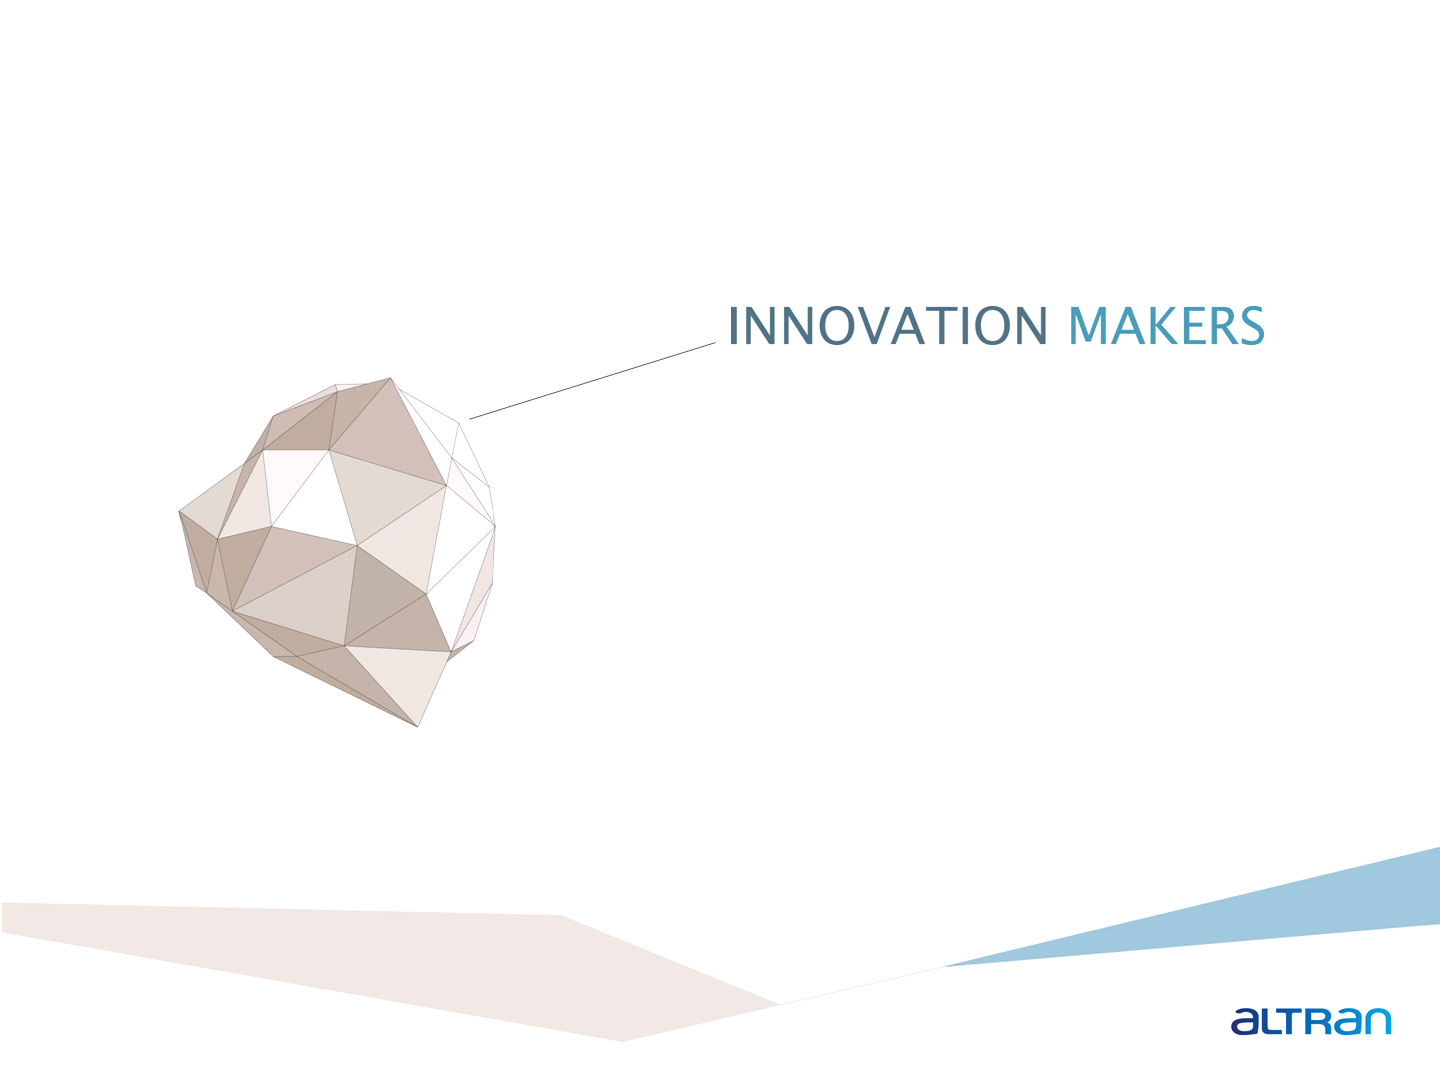
\includegraphics[width=\paperwidth]{pres_back.png}}
  \begin{frame}
  \end{frame}
}
\AtEndDocument{\finalslide}

%\newcommand{\spark}[0]{SPARK}

\DeclareSymbolFont{extraup}{U}{zavm}{m}{n}
\DeclareMathSymbol{\varheart}{\mathalpha}{extraup}{86}

\usepackage{tikz}
\usetikzlibrary{fit}
\usetikzlibrary{arrows}
\usetikzlibrary{calc}
\usetikzlibrary{decorations.pathmorphing}
\usetikzlibrary{shadows}
\usetikzlibrary{shapes.multipart}
\usetikzlibrary{shapes.symbols}

\tikzstyle{files}=[
fill=white,
fill=white,
drop shadow,
draw=AnGrey03,
decorate,
decoration={random steps,segment length=3pt,amplitude=0.5pt},
]

\tikzstyle{tool}=[
draw=AnGrey01,
fill=AnGrey01,
rounded corners
]

\tikzstyle{sa}=[shorten >= 5pt, shorten <= 5pt]

\tikzstyle{pn}=[fill=white,draw=black,text width=1.3cm,text badly centered,drop shadow={fill=AnColour01}]

\tikzstyle{ddg}=[color=AnColour02]
\tikzstyle{tdg}=[color=AnColour01,line width=1pt]
\tikzstyle{paramstyle}=[rectangle,color=AnGrey05,draw,fill=AnGrey01,fill opacity=0.75]


\makeatletter
\newenvironment{btHighlight}[1][]
{\begingroup\tikzset{bt@Highlight@par/.style={#1}}\begin{lrbox}{\@tempboxa}}
{\end{lrbox}\bt@HL@box[bt@Highlight@par]{\@tempboxa}\endgroup}

\newcommand\btHL[1][]{%
  \begin{btHighlight}[#1]\bgroup\aftergroup\bt@HL@endenv%
  \color{white}%
}
\def\bt@HL@endenv{%
  \end{btHighlight}%
  \egroup
}
\newcommand{\bt@HL@box}[2][]{%
  \tikz[#1]{%
    \pgfpathrectangle{\pgfpoint{1pt}{0pt}}{\pgfpoint{\wd #2}{\ht #2}}%
    \pgfusepath{use as bounding box}%
    \node[anchor=base west,fill=AnColour01,outer sep=0pt,inner xsep=1pt, inner ysep=0pt, rounded corners=3pt, minimum height=\ht\strutbox+1pt,#1]{\raisebox{1pt}{\strut}\strut\usebox{#2}};
  }%
}
\makeatother

\lstdefinestyle{magic}{
    basicstyle=\scriptsize\ttfamily,
    moredelim=**[is][\btHL]{`}{`},
}

\author{Florian Schanda}
\title{The \spark 2014 verifying compiler}
\subtitle{A wide and shallow introduction}
\date{October 27, 2015}

\begin{document}

\begin{altrantitle}
  \titleprismlabela{Deductive\\verification}
  \titleprismlabelb{A short\\overview}
  \titleprismlabelc{Florian Schanda}
\end{altrantitle}
%\maketitle

\begin{frame}{So who is \company...}
  \begin{itemize}
  \item \company\ has around $25000$ consultants
  \item In the UK we focus on the development of high-integrity software:
    \begin{itemize}
    \item iFACTS (part of the UK air traffic control)
    \item an engine monitoring unit for a family of commercial aircraft
      engines
    \item etc.
    \end{itemize}
  \item ... and we also develop \spark!
  \end{itemize}
\end{frame}

\begin{frame}{Content}
  \begin{enumerate}
  \item Motivation for static analysis
  \item Ada and \spark: quick history and overview
  \item Architecture + Internals
  \item Conclusion
  \end{enumerate}
\end{frame}

%%%%%%%%%%%%%%%%%%%%%%%%%%%%%%%%%%%%%%%%%%%%%%%%%%%%%%%%%%%%%%%%%%%%%%%%%%%%%%
\section{Introduction}
\begin{frame}{Motivation}{No bugs, please!}
  \begin{center}
    \resizebox{!}{2.7cm}{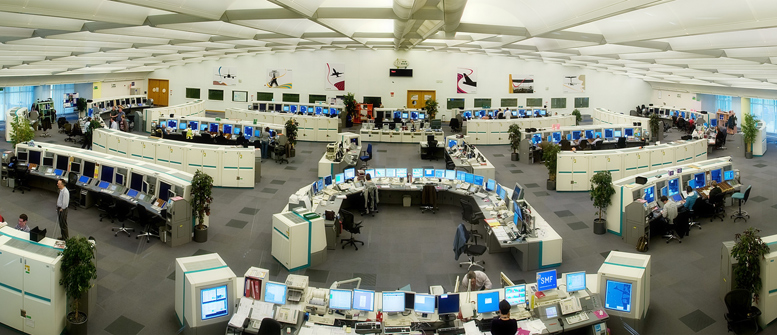
\includegraphics{user_nats.jpg}}
    \resizebox{!}{2.7cm}{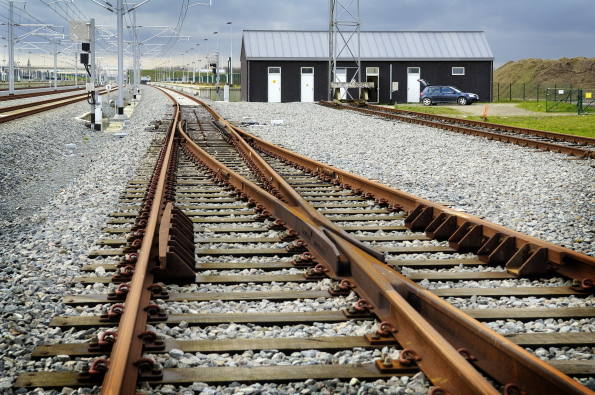
\includegraphics{user_rail.jpg}}
    \resizebox{!}{2.9cm}{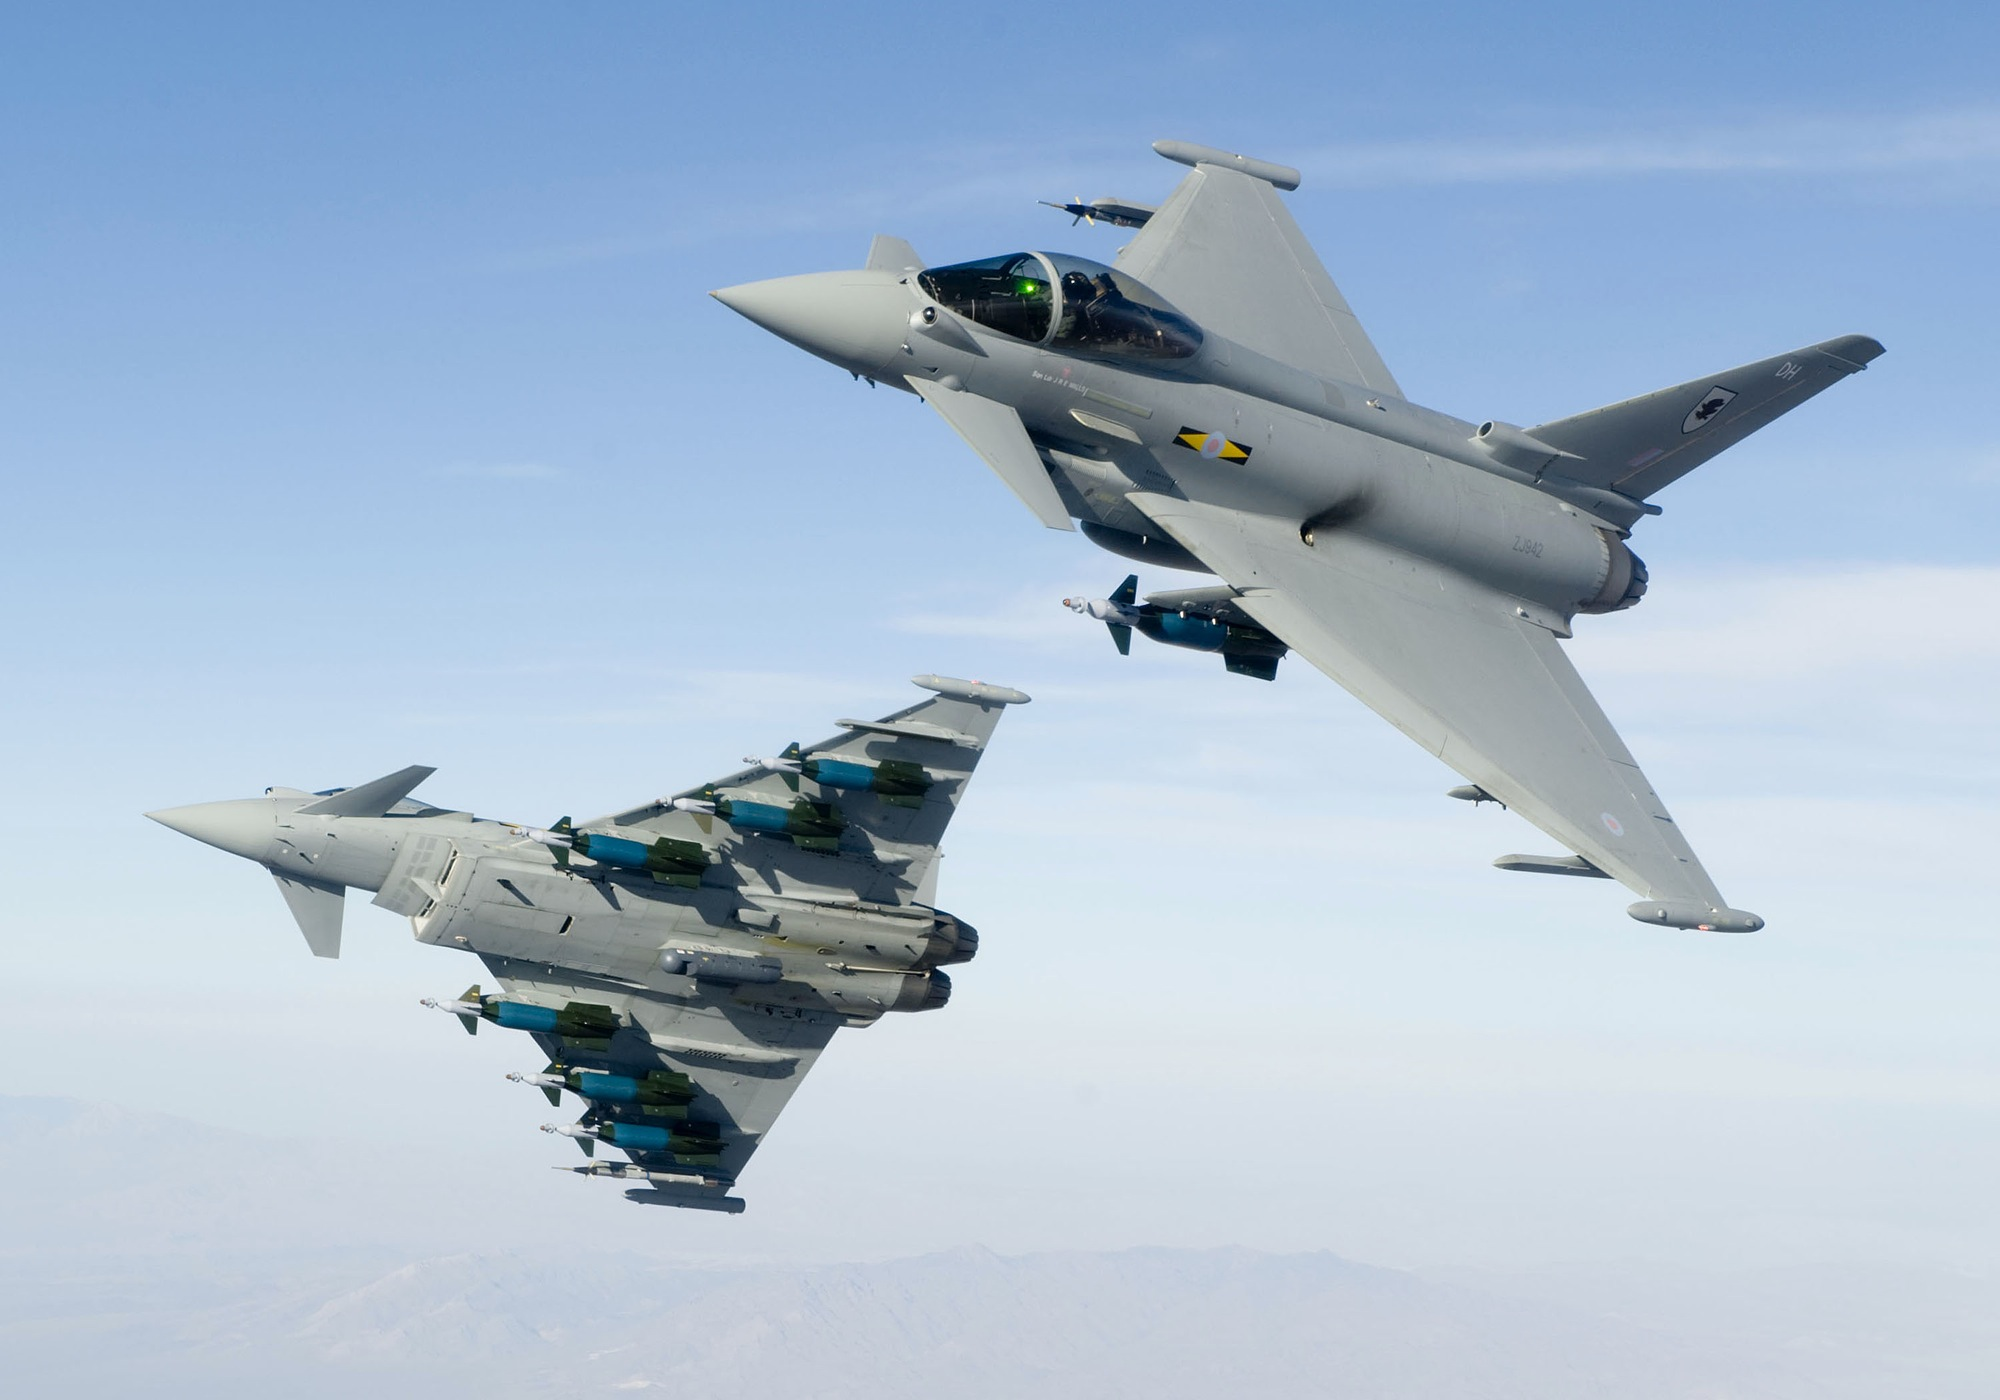
\includegraphics{user_efa.jpg}}
    \resizebox{!}{2.9cm}{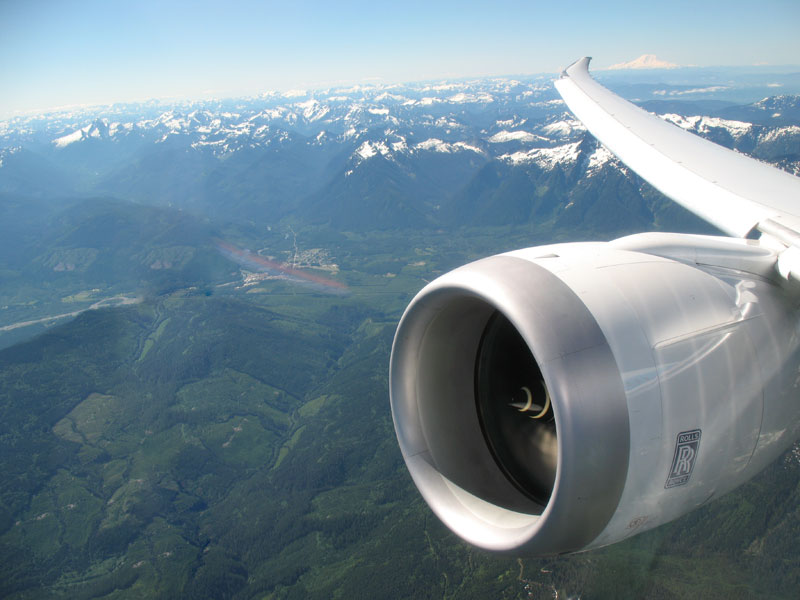
\includegraphics{user_engine.jpg}}
    \resizebox{!}{2.9cm}{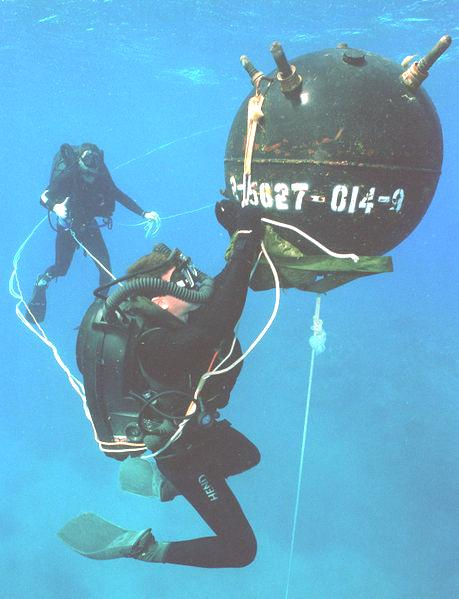
\includegraphics{user_diver.jpg}}
  \end{center}
\end{frame}

\begin{frame}{Motivation}{Otherwise...}
  \begin{center}
    \resizebox{10cm}{!}{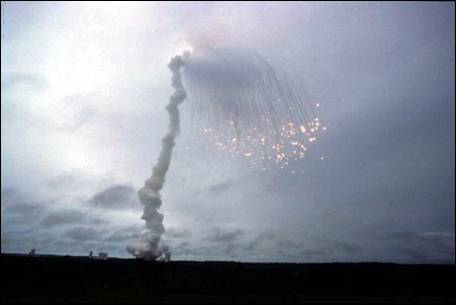
\includegraphics{ariane_5.jpg}}
  \end{center}
\end{frame}

\begin{frame}[fragile]{Static analysis}
  Reason about source code without executing it:
  \begin{pxcode}[language=C,gobble=4]
    int divide_and_fail(int a, int b) {
      return a / b;
    }
  \end{pxcode}
  How many bugs can you find?
  \pause
  \begin{block}{Test 1}
    \begin{pxcode}[language=C,gobble=6]
      result = divide_and_fail(500, 0);
    \end{pxcode}
  \end{block}
  \pause
  \begin{block}{Test 2}
    \begin{pxcode}[language=C,gobble=6]
      result = divide_and_fail(-2147483648, -1);
    \end{pxcode}
  \end{block}
\end{frame}

\begin{frame}[fragile]{Static analysis}
  \begin{itemize}
  \item Testing can only \structure{find} bugs, not prove their absence
  \item Static analysis can be \structure{sound} (no missed bugs)
    \begin{onlyenv}<2->
      \begin{pxcode}[language=bash,gobble=8,showstringspaces=false]
        #!/bin/bash
        echo "your program is wrong"
      \end{pxcode}
    \end{onlyenv}
  \item Static analysis can be \structure{complete} (all alarms are bugs)
    \begin{onlyenv}<3->
      \begin{pxcode}[language=bash,gobble=8,showstringspaces=false]
        #!/bin/bash
        echo "your program is perfect"
      \end{pxcode}
    \end{onlyenv}
  \item Static analysis can be \structure{automatic} (no human intervention)
    \begin{onlyenv}<4->
      \begin{pxcode}[language=bash,gobble=8,showstringspaces=false]
        #!/bin/bash
        echo "potato"
      \end{pxcode}
    \end{onlyenv}
  \end{itemize}
\end{frame}

\begin{frame}{Approaches to static analysis}{Martin's triangle}
  \begin{center}
    \vskip -0.75cm
    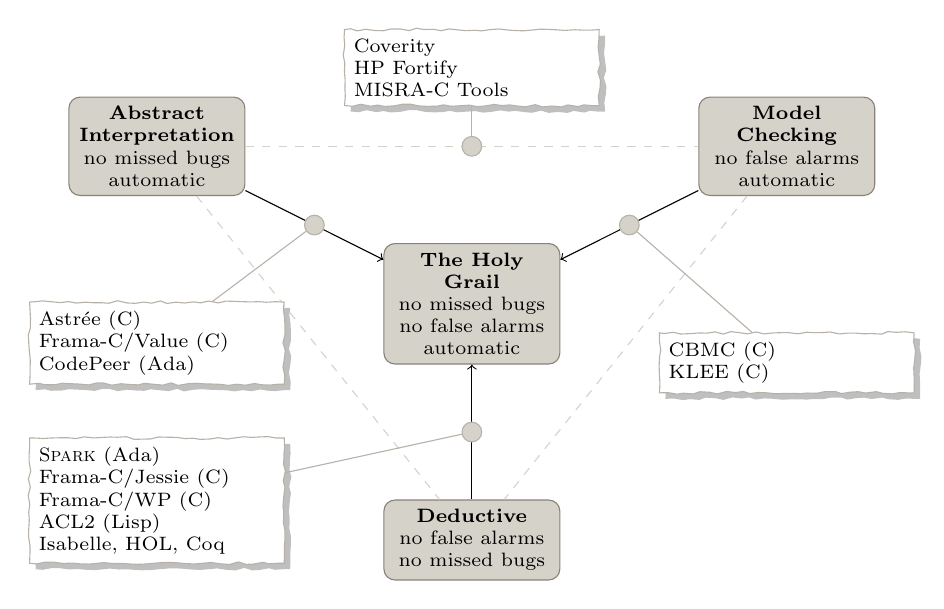
\begin{tikzpicture}
  \tikzstyle{area}=
  [font=\scriptsize,
  text width=2cm,
  draw=AnGrey05,
  rounded corners,
  fill=AnGrey01,
  text badly centered];

  \tikzstyle{descr}=[
  font=\scriptsize,
  text width=3cm,
  fill=white,drop shadow,
  draw=AnGrey03,
  decorate,
  decoration={random steps,segment length=3pt,amplitude=0.5pt},
  ];

  \tikzstyle{link}=
  [draw,
  circle,
  minimum size=2.5mm,
  inner sep=0pt,
  AnGrey03,solid,
  fill=AnGrey01
  ];

  \tikzstyle{tlink}=
  [AnGrey03,
  ];

  \node [area] (deductive) at (0.0, -1.0)
  {
    \textbf{Deductive}\\
    no false alarms\\
    no missed bugs
  };

  \node [area] (model) at (4.0, 4.0)
  {
    \textbf{Model Checking}\\
    no false alarms\\
    automatic
  };

  \node [area] (absint) at (-4.0, 4.0)
  {
    \textbf{Abstract Interpretation}\\
    no missed bugs\\
    automatic
  };

  \node [area] (grail) at (0.0, 2.0)
  {
    \textbf{The Holy Grail}\\
    no missed bugs\\
    no false alarms\\
    automatic
  };

  \draw[AnGrey01,dashed] (absint) -- node [link] (bug_tool_link)   {} (model);
  \draw[AnGrey01,dashed] (absint) -- (deductive);
  \draw[AnGrey01,dashed] (model) -- (deductive);

  \draw[->] (absint)    -- node [link] (ai_tool_link)    {} (grail);
  \draw[->] (model)     -- node [link] (model_tool_link) {} (grail);
  \draw[->] (deductive) -- node [link] (hoare_tool_link) {} (grail);

  \node [descr] (ai_tools) at (-4.0, 1.5)
  {
    Astr\'ee (C)\\
    Frama-C/Value (C)\\
    CodePeer (Ada)
  };

  \node [descr] (hoare_tools) at (-4.0, -0.5)
  {
    \structure{\spark\ (Ada)}\\
    Frama-C/Jessie (C)\\
    Frama-C/WP (C)\\
    ACL2 (Lisp)\\
    Isabelle, HOL, Coq
  };

  \node [descr] (model_tools) at (4.0, 1.25)
  {
    CBMC (C)\\
    KLEE (C)
  };

  \node [descr] (bug_tools) at (0.0, 5.0)
  {
    Coverity\\
    HP Fortify\\
    MISRA-C Tools
  };

  \draw[tlink] (ai_tool_link) -- (ai_tools);
  \draw[tlink] (model_tool_link) -- (model_tools);
  \draw[tlink] (hoare_tool_link) -- (hoare_tools);
  \draw[tlink] (bug_tool_link) -- (bug_tools);
\end{tikzpicture}

  \end{center}
\end{frame}

%%%%%%%%%%%%%%%%%%%%%%%%%%%%%%%%%%%%%%%%%%%%%%%%%%%%%%%%%%%%%%%%%%%%%%%%%%%%%%
\section{Ada and SPARK}
% maybe 10 slides intro
\begin{frame}{What is Ada?}
  \begin{itemize}
  \item Around since 1980
  \item Influenced by ALGOL, Pascal
  \item Emphasis readable code
  \item General purpose, but main users is aerospace and defence
    industry
  \end{itemize}
\end{frame}

\begin{frame}[fragile]{Ada}{Example}
\begin{pxcode}[language=SPARK,gobble=3]
    type U32 is mod 2 ** 32;

    procedure Swap (A, B : in out U32)
    is
       Tmp : U32;
    begin
       Tmp := A;
       A   := B;
       B   := Tmp;
    end Swap;
\end{pxcode}
\end{frame}

\begin{frame}{What is \spark?}
  It is a \structure{language} and a \structure{toolset}.
  \begin{itemize}
  \item The language is a variant of Ada:
    \begin{itemize}
    \item unsafe and difficult constructs excluded
    \item contracts
    \item reference manual publicly available (GFDL)
    \end{itemize}
  \item The toolset is a \structure{static analysis} tool
    \begin{itemize}
    \item sound, but with a low false alarm rate
    \item deductive
    \item publicly available (GPL3)
    \end{itemize}
    \pause
  \item ...and it's actually \structure{used in real life}
  \end{itemize}
\end{frame}

\begin{frame}{What is \spark?}{A brief history}
  \begin{description}
  \item[1985] University of Southampton - SPADE
  \item[1987] PVL, Praxis, Altran - \spark\ 83, 95, 2005
  \item[2011] Altran + AdaCore - GPLv3 release of \spark
  \item[2013] Altran + AdaCore - \spark 2014
  \end{description}
\end{frame}

\begin{frame}[fragile]{What is \spark?}{An example}
  \begin{pxcode}[language=SPARK,gobble=4]
    type U32 is mod 2 ** 32;

    procedure Swap (A, B : in out U32)
    with
       Global => null,
       Post   => A = B'Old and
                 B = A'Old
    is
    begin
       A := A xor B;
       B := A xor B;
       A := A xor B;
    end Swap;
  \end{pxcode}
\end{frame}

\begin{frame}[fragile]{What is \spark?}{Another example}
  \begin{pxcode}[language=SPARK,gobble=4]
    type Int_Array is array (1 .. 10) of Integer;

    procedure Find_Element (A     : in     Int_Array;
                            Elem  : in     Integer;
                            Idx   :    out Natural;
                            Found :    out Boolean)
    with
       Post => (if Found then A (Idx) = Elem)
    is
    begin
       for I in A'Range loop
          Idx   := I;
          Found := A (I) = Elem;
          exit when Found;
       end loop;
    end Find_Element;
  \end{pxcode}
\end{frame}

\begin{frame}[fragile]{What is \spark?}{Headline features}
  \begin{itemize}
  \item Strong typing
    \begin{pxcode}[language=SPARK,gobble=6]
      type Grams  is new Float range 0.0 .. 100.0;
      type Pounds is new Float range 0.0 .. 100.0;
    \end{pxcode}

  \item Many contracts...
    \begin{itemize}
    \item Parameter modes (in, in out, out)
    \item Globals, Depends, Abstract\_State
    \item Pre, Post, Contract\_Cases
    \item No\_Return, Volatile, Atomic
    \item Asserts, Invariants, Variants
    \end{itemize}
    ...most of which are \structure{executable}

  \item Ghost code

  \item No pointers (or aliasing), instead:
    \begin{itemize}
    \item Pass by reference
    \item Container library
    \end{itemize}
  \item No side-effects
  \end{itemize}
\end{frame}

\begin{frame}[fragile]{What is \spark?}{The tools}
  \begin{itemize}
  \item Developed jointly at Altran (Bath) and AdaCore (Paris, and
    more)
    \begin{itemize}
    \item 4 in Bath
    \item 5 in Paris
    \item plus more (language design, gcc, etc.)
    \end{itemize}
  \item Based on free software (gcc, Why3, CVC4, etc.)
  \item Based on published results, and ongoing collaborations with
    universities
  \item Very fun!
  \end{itemize}
\end{frame}


%%%%%%%%%%%%%%%%%%%%%%%%%%%%%%%%%%%%%%%%%%%%%%%%%%%%%%%%%%%%%%%%%%%%%%%%%%%%%%
\section{Architecture}
% maybe 5 slides

\begin{frame}{Tool architecture}{User view}
  \begin{center}
    
\begin{tikzpicture}[x=3cm,y=1.5cm,sa]

      \node[files] (source)    at (0, 0) {Source};
      \node[tool]  (gnatprove) at (1, 0) {gnatprove};
      \node        (output)    at (2, 0) {Verdict};

      \draw[->] (source) -- (gnatprove);
      \draw[->] (gnatprove) -- (output);
    \end{tikzpicture}
  \end{center}
\end{frame}

\begin{frame}{Tool architecture}{More detailed view...}
  \begin{center}
    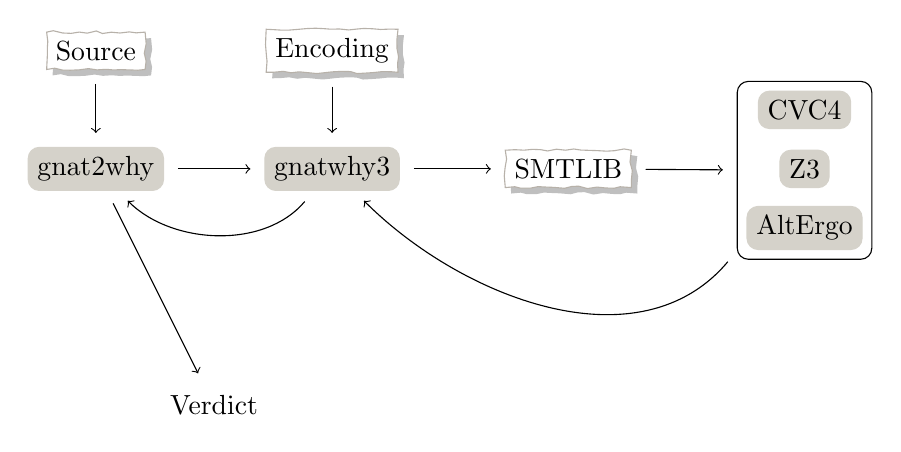
\begin{tikzpicture}[x=3cm,y=1.5cm,sa]
      \node[tool] (gnat2why) at (1, 0) {gnat2why};
      \node[tool] (gnatwhy3) at (2, 0) {gnatwhy3};
      \node[files] (smt) at (3, 0) {SMTLIB};

      \node[tool] (cvc4)    at (4, 0.5)  {CVC4};
      \node[tool] (z3)      at (4, 0)  {Z3};
      \node[tool] (altergo) at (4, -0.5) {AltErgo};

      \node[draw,
            fit=(cvc4)(z3)(altergo),
            rounded corners
            ] (provers) {};

      \draw[->] (gnat2why) -- (gnatwhy3);
      \draw[->] (gnatwhy3) -- (smt);
      \draw[->] (smt)      -- (provers);

      \node[files] (source) at (1, 1) {Source};
      \node[files] (encoding) at (2, 1) {Encoding};

      \node (output) at (1.5, -2) {Verdict};

      \draw[->] (source) -- (gnat2why);
      \draw[->] (encoding) -- (gnatwhy3);

      \draw[->] (gnat2why) -- (output);
      \draw[->] (gnatwhy3) to [out=230,in=-45] (gnat2why);

      \draw[->] (provers) to [out=230,in=-45] (gnatwhy3);
    \end{tikzpicture}
  \end{center}
\end{frame}

\begin{frame}{Tool architecture}{gnat2why}
  This is what we \structure{develop ourselves}.
  \begin{itemize}
  \item Contains \spark/Ada parser
  \item Does some preliminary analysis
  \item Compilation to intermediate language
  \end{itemize}
  Other tools are also free software that are used by us and others.
\end{frame}

%%%%%%%%%%%%%%%%%%%%%%%%%%%%%%%%%%%%%%%%%%%%%%%%%%%%%%%%%%%%%%%%%%%%%%%%%%%%%%
\section{Internals}
\subsection{Parsing SPARK}
\begin{frame}{GNAT Frontend}{Overview}
  \begin{itemize}
  \item Ada 2012 and \spark 2014 lexer,
  \item parser,
  \item semantic analyser,
  \item expander,
  \item code generator (with gcc via intermediate language)
  \end{itemize}
\end{frame}

\begin{frame}{GNAT Frontend}{Lexer and Parser}
  \begin{itemize}
  \item Hand-written lexer
  \item Hand-written parser, recursive descent, with arbitrary look-ahead
    \begin{itemize}
    \item better error messages, especially for serious structural
      errors
    \item closely aligned with published Ada RM grammar
    \end{itemize}
  \item Produces AST
    \begin{itemize}
    \item Nodes (structure of program)
    \item Entities (identifiers, operator symbols, etc.)
    \end{itemize}
  \item There is no classical symbol table
  \item Entities \structure{are} the symbol table
  \end{itemize}
\end{frame}

\begin{frame}[fragile]{GNAT Frontend}{The AST}
  \begin{itemize}
  \item Table indexed by integers (so no pointers as such)
  \item No OO, instead records with generic fields (field1, field2,
    field3, etc.) and access subprograms that give them meaning based
    on node type:
    \begin{pxcode}[language=SPARK,gobble=6]
      function Etype              (N : Node_Id) return Node_Id;
      function Exception_Choices  (N : Node_Id) return List_Id;
      function Exception_Handlers (N : Node_Id) return List_Id;
      ...
    \end{pxcode}
  \item 12,000+ line comment that is \structure{tool-enforced} for
    documentation
  \end{itemize}
\end{frame}

\begin{frame}[fragile]{GNAT Frontend}{AST example}
Partial tree for \verb|return a / b;|
\begin{pxcode}[style=tinystyle]
Node #1 N_Simple_Return_Statement (Node_Id=2346) (source,analyzed)
 Sloc = 8249  foo.adb:4:4
 Return_Statement_Entity = Node #5 N_Defining_Identifier "R1b" (Entity_Id=2350)
 Expression = Node #2 N_Op_Divide "Odivide" (Node_Id=2347)

  Node #2 N_Op_Divide "Odivide" (Node_Id=2347) (source,analyzed)
   Parent = Node #1 N_Simple_Return_Statement (Node_Id=2346)
   Sloc = 8258  foo.adb:4:13
   Chars = "Odivide" (Name_Id=300000413)
   Left_Opnd = Node #3 N_Identifier "a" (Node_Id=2345)
   Right_Opnd = Node #4 N_Identifier "b" (Node_Id=2348)
   Entity = N_Defining_Identifier "Odivide" (Entity_Id=1919s)
   Do_Overflow_Check = True
   Etype = N_Defining_Identifier "integer" (Entity_Id=1035s)
   Do_Division_Check = True

    Node #3 N_Identifier "a" (Node_Id=2345) (source,analyzed)
     Parent = Node #2 N_Op_Divide "Odivide" (Node_Id=2347)
     Sloc = 8256  foo.adb:4:11
     Chars = "a" (Name_Id=300000099)
     Etype = N_Defining_Identifier "integer" (Entity_Id=37s)
     Entity = N_Defining_Identifier "a" (Entity_Id=2324)
     Associated_Node = N_Defining_Identifier "a" (Entity_Id=2324)

    ...
\end{pxcode}
\end{frame}

\begin{frame}[fragile]{GNAT Frontend}{The expander and code generation}
  \begin{itemize}
  \item Generics are expanded here
  \item Also deals with tasks, protected objects and object orientation
  \item AST is transformed to something the GCC code generator expects
  \end{itemize}
\end{frame}

% 5-10 slides

\subsection{Translation to IL}
\begin{frame}{gnat2why}{Overview}
  \begin{itemize}
  \item Just another GNAT back-end
  \item An elaborate semantic analysis pass over the AST:
    \begin{description}
    \item[filter] Note which areas of the program are ``in \spark''
    \item[globals] Generate frame conditions (global contracts if they
      have not been specified) at varying levels of details
    \item[flow] Check initialization, non-aliasing, global contracts,
      and information flow contracts
    \item[translation] Transform \spark\ subprograms into WhyML
      subprograms
    \end{description}
  \end{itemize}
\end{frame}

\begin{frame}{gnat2why}{Overview}
  \begin{center}
    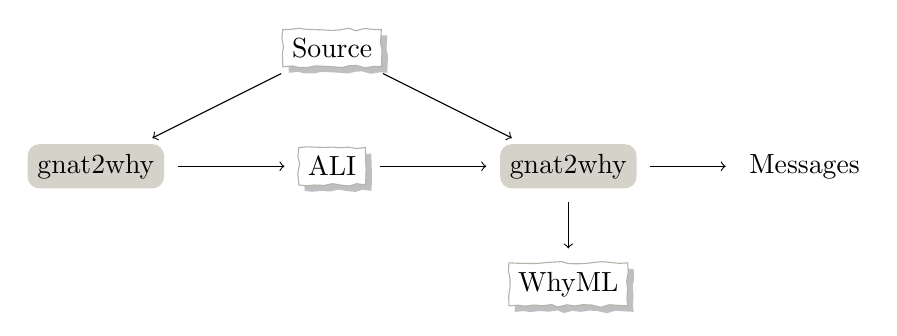
\begin{tikzpicture}[x=3cm,y=-1.5cm,sa]
      \node[files] (source)   at (0, 0) {Source};
      \node[tool]  (phase1)   at (-1, 1) {gnat2why};
      \node[files] (ali)      at (0, 1) {ALI};
      \node[tool]  (phase2)   at (1, 1) {gnat2why};
      \node        (messages) at (2, 1) {Messages};
      \node[files] (why3)     at (1, 2) {WhyML};

      \draw[->] (source) -- (phase1);
      \draw[->] (source) -- (phase2);
      \draw[->] (phase1) -- (ali);
      \draw[->] (ali) -- (phase2);
      \draw[->] (phase2) -- (messages);
      \draw[->] (phase2) -- (why3);
    \end{tikzpicture}
  \end{center}
\end{frame}

\begin{frame}[fragile]{gnat2why}{Filter}
  \begin{itemize}
  \item Useful for analysing programs partly in \spark, partly in Ada
  \item Essentially assigns Boolean flag to all entities
  \item Produces error messages if things \structure{have} to be in
    \spark
  \item Fairly obvious top-down tree-walk
  \end{itemize}
  \begin{block}{Example}
    \begin{pxcode}[language=SPARK,gobble=6]
      package P1 is
         type T1 is range 1 .. 10;  -- T in SPARK
         type T2 is access Float;   -- T2 not in SPARK
      end P1;

      package P2 with SPARK_Mode is
         type T3 is access Integer; -- ERROR
      end P2;
    \end{pxcode}
  \end{block}
\end{frame}

\begin{frame}{gnat2why}{Flow}
  \begin{itemize}
  \item Over-approximation, automatic
  \item More or less implements ``system dependence graphs''
  \item Checks initialization of all variables
    \begin{itemize}
    \item an important assumption for proof
    \item an important check for information leaks
    \end{itemize}
  \item Checks non-aliasing, an important assumption for proof
  \item Determines or checks frame conditions
  \item Checks flow contracts
  \item Checks for data races (for tasking)
  \item Warns of some suspicious constructs (ineffective code, etc.)
  \end{itemize}
\end{frame}

\begin{frame}{gnat2why}{Flow}
  \begin{center}
    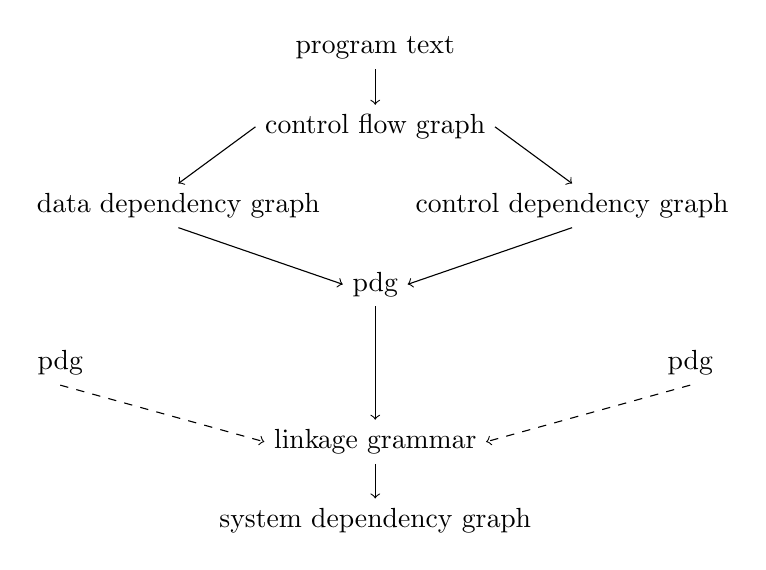
\begin{tikzpicture}
      \node[name=ptext] at (0,     0)  {program text};
      \node[name=cfg]   at (0,    -1)  {control flow graph};
      \node[name=ddg]   at (-2.5, -2)  {data dependency graph};
      \node[name=cdg]   at (2.5,  -2)  {control dependency graph};
      \node[name=pdg]   at (0,    -3)  {pdg};
      \node[name=pdg_b] at (-4,   -4)  {pdg};
      \node[name=pdg_c] at (4,    -4)  {pdg};
      \node[name=lg]    at (0,    -5)  {linkage grammar};
      \node[name=sdg]   at (0,    -6)  {system dependency graph};

      \draw ($(ptext.south)$) edge[->] ($(cfg.north)$);
      \draw ($(cfg.west)$)    edge[->] ($(ddg.north)$);
      \draw ($(cfg.east)$)    edge[->] ($(cdg.north)$);
      \draw ($(ddg.south)$)   edge[->] ($(pdg.west)$);
      \draw ($(cdg.south)$)   edge[->] ($(pdg.east)$);
      \draw ($(pdg.south)$)   edge[->] ($(lg.north)$);
      \draw ($(pdg_b.south)$) edge[->, dashed] ($(lg.west)$);
      \draw ($(pdg_c.south)$) edge[->, dashed] ($(lg.east)$);
      \draw ($(lg.south)$)    edge[->] ($(sdg.north)$);
    \end{tikzpicture}
  \end{center}
\end{frame}

\begin{frame}[fragile]{gnat2why}{Flow - Control flow graph}
  \begin{columns}[c]
    \begin{column}{2cm}
      \begin{pxcode}[language=Ada,gobble=8]
        if a then
           x := 0;
        else
           return;
        end if;
        y := 0;
      \end{pxcode}
    \end{column}
    \begin{column}{2cm}
      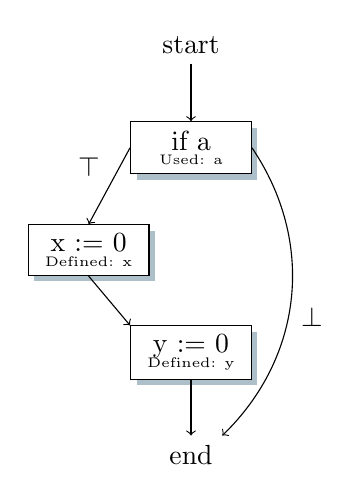
\begin{tikzpicture}[scale=1.3]
        \node[name=start] at (0,0)          {start};
        \node[pn, name=if_a] at (0,-1)      {if a\tiny\\\vskip-1em Used: a};
        \node[pn, name=x_set_0] at (-1, -2) {x := 0\tiny\\\vskip-1em Defined: x};
        \node[pn, name=y_set_0] at (0, -3)  {y := 0\tiny\\\vskip-1em Defined: y};
        \node[name=end] at (0,-4)           {end};

        \draw ($(start.south)$) edge[->] ($(if_a.north)$);
        \draw ($(if_a.west)$) edge[->] node[auto,swap] {$\top$} ($(x_set_0.north)$);
        \draw ($(if_a.east)$) edge[->, bend left=40] node[auto] {$\bot$} ($(end.north east)$);
        \draw ($(x_set_0.south)$) edge[->] ($(y_set_0.north west)$);
        \draw ($(y_set_0.south)$) edge[->] ($(end.north)$);
      \end{tikzpicture}
    \end{column}
  \end{columns}
\end{frame}

\begin{frame}{gnat2why}{Flow - Data dependence graph}
  \begin{columns}[c]
    \begin{column}{2cm}
      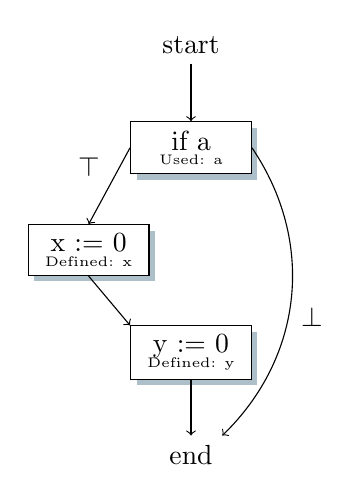
\begin{tikzpicture}[scale=1.3]
        \node[name=start] at (0,0)          {start};
        \node[pn, name=if_a] at (0,-1)      {if a\tiny\\\vskip-1em Used: a};
        \node[pn, name=x_set_0] at (-1, -2) {x := 0\tiny\\\vskip-1em Defined: x};
        \node[pn, name=y_set_0] at (0, -3)  {y := 0\tiny\\\vskip-1em Defined: y};
        \node[name=end] at (0,-4)           {end};

        \draw ($(start.south)$) edge[->] ($(if_a.north)$);
        \draw ($(if_a.west)$) edge[->] node[auto,swap] {$\top$} ($(x_set_0.north)$);
        \draw ($(if_a.east)$) edge[->, bend left=40] node[auto] {$\bot$} ($(end.north east)$);
        \draw ($(x_set_0.south)$) edge[->] ($(y_set_0.north west)$);
        \draw ($(y_set_0.south)$) edge[->] ($(end.north)$);
      \end{tikzpicture}
    \end{column}
    \begin{column}{5cm}
      Def-use chains:
      \begin{itemize}
      \item $a$
        \begin{itemize}
        \item start $\rightarrow$ if a
        \item start $\rightarrow$ end
        \end{itemize}
      \item $x$
        \begin{itemize}
        \item start $\rightarrow$ end
        \item x := 0 $\rightarrow$ end
        \end{itemize}
      \item $y$
        \begin{itemize}
        \item start $\rightarrow$ end
        \item y := 0 $\rightarrow$ end
        \end{itemize}
      \end{itemize}
    \end{column}
  \end{columns}
\end{frame}

\begin{frame}{gnat2why}{Flow - Data dependence graph}
  We can now draw the DDG:
  \begin{center}
    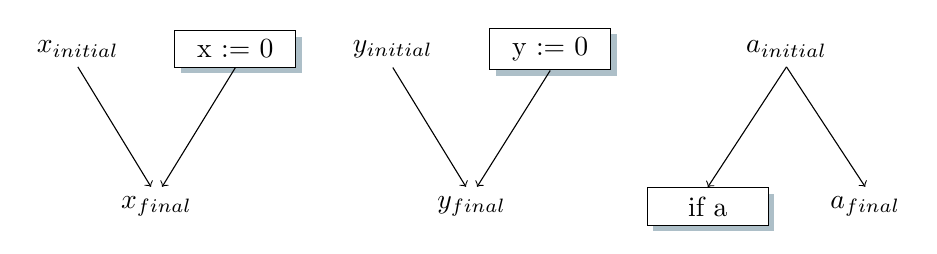
\begin{tikzpicture}[scale=2]
      \node[name=x_initial] at (0,0) {$x_{initial}$};
      \node[name=x_set_0,pn]   at (1,0) {x := 0};
      \node[name=y_initial] at (2,0) {$y_{initial}$};
      \node[name=y_set_0,pn]   at (3,0) {y := 0};
      \node[name=a_initial] at (4.5,0) {$a_{initial}$};

      \node[name=x_final]   at (0.5,-1) {$x_{final}$};
      \node[name=y_final]   at (2.5,-1) {$y_{final}$};
      \node[name=if_a,pn]      at (4,-1) {if a};
      \node[name=a_final]   at (5,-1) {$a_{final}$};

      \draw ($(x_initial.south)$) edge[->] ($(x_final.north)-(1pt,0)$);
      \draw ($(x_set_0.south)$) edge[->] ($(x_final.north)+(1pt,0)$);
      \draw ($(y_initial.south)$) edge[->] ($(y_final.north)-(1pt,0)$);
      \draw ($(y_set_0.south)$) edge[->] ($(y_final.north)+(1pt,0)$);
      \draw ($(a_initial.south)$) edge[->] ($(a_final.north)$);
      \draw ($(a_initial.south)$) edge[->] ($(if_a.north)$);
    \end{tikzpicture}
  \end{center}
\end{frame}

\begin{frame}[fragile]{gnat2why}{Flow - Control dependence graph}
  \begin{columns}[c]
    \begin{column}{2cm}
      \begin{pxcode}[language=Ada,gobble=8]
        if a then
           x := 0;
        else
           return;
        end if;
        y := 0;
      \end{pxcode}
    \end{column}
    \begin{column}{4cm}
      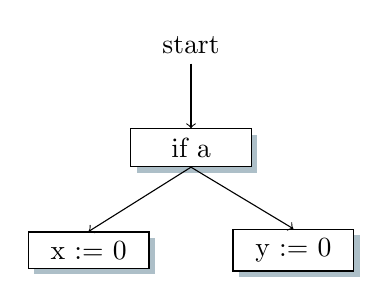
\begin{tikzpicture}[scale=1.3]
        \node[name=start] at (0,0)          {start};
        \node[pn, name=if_a] at (0,-1)      {if a};
        \node[pn, name=x_set_0] at (-1, -2) {x := 0};
        \node[pn, name=y_set_0] at ( 1, -2) {y := 0};

        \draw ($(start.south)$) edge[->] ($(if_a.north)$);
        \draw ($(if_a.south)$) edge[->] ($(x_set_0.north)$);
        \draw ($(if_a.south)$) edge[->] ($(y_set_0.north)$);
      \end{tikzpicture}
    \end{column}
  \end{columns}
  \vskip 1cm
  Algorithm: produce dominance frontier of the reversed control flow
  graph (``post dominance frontier'').
\end{frame}

\begin{frame}{gnat2why}{Flow - Program dependence graph}
  To construct the program dependence graph (\structure{PDG}) we
  simply overlay the CDG and DDG.

  \begin{center}
    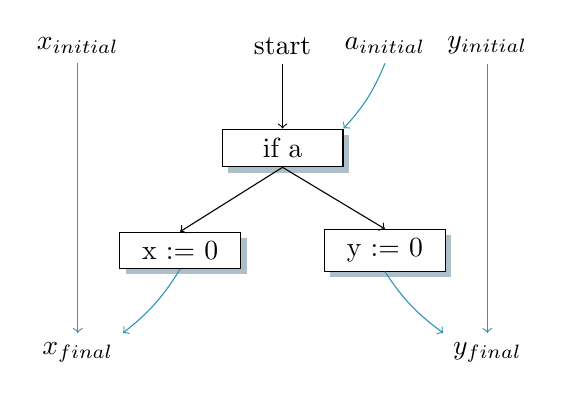
\begin{tikzpicture}[scale=1.3]
      \node[name=start] at (0,0)          {start};
      \node[pn, name=if_a] at (0,-1)      {if a};
      \node[pn, name=x_set_0] at (-1, -2) {x := 0};
      \node[pn, name=y_set_0] at ( 1, -2) {y := 0};

      \node[name=a_initial] at  (1, 0)     {$a_{initial}$};
      \node[name=x_initial] at (-2, 0)     {$x_{initial}$};
      \node[name=y_initial] at ( 2, 0)     {$y_{initial}$};

      \node[name=x_final] at (-2, -3)     {$x_{final}$};
      \node[name=y_final] at ( 2, -3)     {$y_{final}$};

      \draw ($(start.south)$) edge[->] ($(if_a.north)$);
      \draw ($(if_a.south)$) edge[->] ($(x_set_0.north)$);
      \draw ($(if_a.south)$) edge[->] ($(y_set_0.north)$);

      \draw ($(x_initial.south)$) edge[->, ddg] ($(x_final.north)$);
      \draw ($(y_initial.south)$) edge[->, ddg] ($(y_final.north)$);

      \draw ($(a_initial.south)$) edge[->, ddg, bend left=10] ($(if_a.north east)$);

      \draw ($(x_set_0.south)$) edge[->, ddg, bend left=10] ($(x_final.north east)$);
      \draw ($(y_set_0.south)$) edge[->, ddg, bend right=10] ($(y_final.north west)$);
    \end{tikzpicture}
  \end{center}
\end{frame}

\begin{frame}{gnat2why}{Flow}
  \begin{itemize}
  \item There is much more detail in flow:
    \begin{itemize}
    \item Inter-procedural analysis and recursion
    \item Non-terminating subprograms
    \item Tasking
    \item Component-level analysis of records
    \item Volatile variables
    \item etc.
    \end{itemize}
  \item Debug output is done through \structure{graphviz} and has been
    a \structure{primary} design concern
  \end{itemize}
\end{frame}

% TODO: flow error examples?

\begin{frame}{gnat2why}{Translation to WhyML}
  \begin{itemize}
  \item \spark\ is still an extremely complicated language
  \item Key properties need to be proven for a program to be correct
    (``verification conditions'', or ``VCs'')
  \item Translation to a smaller, intermediate language WhyML
    \begin{itemize}
    \item Simpler control flow
    \item Simpler types
    \end{itemize}
  \item Verification condition generation based on this IL
  \end{itemize}
\end{frame}

\begin{frame}[fragile]{gnat2why}{Translation to WhyML}
\begin{columns}[c]
\begin{column}{3cm}
  \begin{pxcode}[language=SPARK,gobble=4]
    function Example
       (A, B : Natural)
        return Natural
    is
       R : Natural;
    begin
       if A < B then
          R := A + 1;
       else
          R := B - 1;
       end if;
       return R;
    end Example;
  \end{pxcode}
\end{column}
\pause
\begin{column}{0.3cm}
  $\rightarrow$
\end{column}
\begin{column}{7cm}
\begin{pxcode}[language=ML]
let example (a: int) (b: int)
    requires { a >= 0 /\ a <= 2147483647 }
    requires { b >= 0 /\ b <= 2147483647 }
    returns { r -> r >= 0 /\
                   r <= 2147483647 }
  = let r = ref 0 in
    if a < b then
       r := a + 1
    else
       r := b - 1;
    (!r)
\end{pxcode}
\end{column}
\end{columns}
\end{frame}

\begin{frame}{gnat2why}{Translation to WhyML}
  \begin{itemize}
  \item Another traversal over AST (for \spark), building another AST
    (for Why3)
  \item Tree is ``pretty'' printed, but not meant to be human readable
  \item One or more Why3 modules per \spark\ entity
    \begin{itemize}
    \item Types
    \item Entity definitions, axioms
    \item Subprogram definitions, axioms, bodies
    \end{itemize}
    All of which are dumped into a single file for \texttt{gnatwhy3}.
  \item Not as nice as the previous example, a lot of extra
    information embedded:
    \begin{itemize}
    \item Original source locations of all VCs
    \item Checks ($x \ne 0$, or $x < 2^{32}$, etc.)
    \end{itemize}
  \end{itemize}
\end{frame}

\begin{frame}[fragile]{gnat2why}{Translation to WhyML}
Yep, not very readable... VC fragment for $r = a / b$:
\begin{pxcode}[style=magic]
( ( "GP_Sloc:overflow.adb:7:7" ( #"overflow.adb" 7 0 0#
overflow__example__result.int__content <- ( (
#"overflow.adb" 7 0 0# "GP_Sloc:overflow.adb:7:16"
"GP_Shape:return__div" "keep_on_simp" "model_vc"
"GP_Reason:VC_OVERFLOW_CHECK" "GP_Id:1"
(Standard__integer.range_check_(( #"overflow.adb" 7 0 0#
"GP_Reason:VC_DIVISION_CHECK" "GP_Id:0"
"GP_Sloc:overflow.adb:7:16" "GP_Shape:return__div"
"keep_on_simp" "model_vc" `(Int_Division.div_`
`(Overflow__example__a.a) (Overflow__example__b.b))`
))) ) ); #"overflow.adb" 7 0 0# raise Return__exc ) );
#"overflow.adb" 3 0 0# raise Return__exc )
\end{pxcode}
\pause
\begin{block}{But we eventually get nice output...}
\scriptsize
overflow.adb:7:16: medium: divide by zero might fail (e.g. when B = 0)\\
overflow.adb:7:16: medium: overflow check might fail
\end{block}
\end{frame}

\begin{frame}{gnat2why}{Translation to WhyML}
  Features of the IL:
  \begin{itemize}
  \item Based on first order logic + theories
  \item In vague ML syntax with programming constructs:
    \begin{itemize}
    \item (mutable) variables
    \item sequences
    \item loops, if, etc.
    \item assertions
    \item exceptions
    \end{itemize}
  \item Built-in types are Boolean, Int, Real, Arrays, Records, Lists,
    Sets, etc. but more can be defined
  \end{itemize}
\end{frame}

\begin{frame}{gnat2why}{Translation to WhyML}
  All checks come from a specification:
  \begin{itemize}
  \item Some checks are user defined (user asserts, postconditions)
  \item Ada RM defines basic checks (overflow, range, index, division
    by zero, discriminants, etc.)
  \item \spark\ RM defines more (LSP checks, loop variants and
    invariants, etc.)
  \end{itemize}
  ... we just follow that spec, and err on side of redundant checks.
\end{frame}

% QUESTION: should I include something about gnatprove here
%\subsection{gnatprove}
% 1-2 slides

\subsection{SMT}
\begin{frame}{SAT, SMT and SMTLIB}
  Recap: we now have the \spark\ program in a different language (WhyML),
  but have not verified much...
  \begin{itemize}
  \item It's still difficult to prove anything, so we need to start talking
    to (automatic) theorem provers
  \item Language of choice is SMTLIB, but others exist
  \item So, next step is \structure{another} language transformation
  \item But, to appreciate this step, let's first talk about SMT...
  \end{itemize}
\end{frame}

\begin{frame}{SAT, SMT and SMTLIB}{Recap of SAT}
  Let's start with SAT:
  \begin{itemize}
  \item Is there an assignment for $(a \lor \lnot c) \land (\lnot b
    \lor c) \land (d)$ that makes everything true?
    \pause
  \item Yes, at least one: $\lnot a, \lnot b, \lnot c, d$
  \item Significant advances in the last 15 years
  \item Modern CDCL\footnote{conflict-driven clause learning} solvers
    can solve \structure{huge} problems with millions of variables
  \end{itemize}
\end{frame}

\begin{frame}{SAT, SMT and SMTLIB}{Overview of SMT}
  SAT modulo theories: SMT
  \begin{itemize}
  \item Is some first-order logic formula SAT (given some background
    theory)?
    \pause
  \item $(0 \varheart x) \land (0 \varheart y) \land
    (x \spadesuit y \varheart x)$ \pause
  \item We need an interpretation for $\varheart$ and $\spadesuit$ to
    decide!
    \pause
  \item $\varheart = <$ and $\spadesuit = +$ and
    $D = \mathbb{R}$:\\
    $(0 < x) \land (0 < y) \land (x + y < x)$
    \pause - {\color{AnSecondary01} UNSAT}
    \pause
  \item $\varheart = <$ and $\spadesuit = +_{mod 256}$ and
    $D = uint8\_t$:\\
    $(0 < x) \land (0 < y) \land (x +_{mod 256} y < x)$
    \pause - {\color{AnSecondary01} SAT ($x = 255$, $y = 1)$}
  \end{itemize}
\end{frame}

\begin{frame}{SAT, SMT and SMTLIB}{SMT Example}
  \begin{itemize}
  \item<1-> $(0 < x) \land (0 < y) \land (x + y < x)$
  \item<2-> Is this SAT? $A_1 \land A_2 \land A_3$
  \item<3-> YES - ($A_1, A_2, A_3$)
  \item<4-> Hand over to theory solver:\\
    $0 < x$\\
    $0 < y$\\
    \only<4>{$x + y < x$}
    \only<5>{$x + y < x$  (substract by $x$)}
    \only<6>{$y < 0$}
    \only<7->{$y < 0$ (contradiction between $A_2$ and $A_3$!)}
  \item<8-> Add $\lnot (A_2 \land A_3)$ to the SAT problem
  \item<9-> Is this SAT? $A_1 \land A_2 \land A_3 \land (\lnot A_2 \lor
    \lnot A_3)$
  \item<10-> UNSAT
  \end{itemize}
\end{frame}

\begin{frame}{SAT, SMT and SMTLIB}{Architecture of modern SMT solver (thanks to Liana for the picture)}
  \begin{center}
    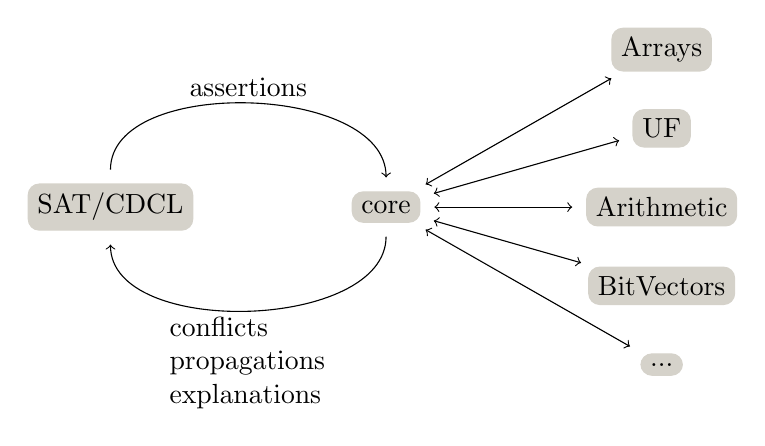
\begin{tikzpicture}[x=3.5cm,sa]
      \node[tool] (cdcl) at (0, 0) {SAT/CDCL};
      \node[tool] (core) at (1, 0) {core};

      \draw[->] (cdcl) to[out=90,in=90] node[auto]{assertions} (core);
      \draw[->] (core) to[out=-90,in=-90]
                       node[auto,text width=2cm]
                       {conflicts\\propagations\\explanations}
                (cdcl);

      \node[tool] (arrays) at (2, 2) {Arrays};
      \node[tool] (uf)     at (2, 1) {UF};
      \node[tool] (lra)    at (2,  0) {Arithmetic};
      \node[tool] (bv)     at (2,  -1) {BitVectors};
      \node[tool] (other)  at (2,  -2) {...};

      \draw[<->] (core) -- (arrays);
      \draw[<->] (core) -- (uf);
      \draw[<->] (core) -- (lra);
      \draw[<->] (core) -- (bv);
      \draw[<->] (core) -- (other);
    \end{tikzpicture}
  \end{center}
\end{frame}

\begin{frame}{SAT, SMT and SMTLIB}{Theories}
  Many theories have been implemented:
  \begin{itemize}
  \item Boolean
  \item Integer
  \item Reals
  \item Quantifiers
  \item Arrays
  \item Uninterpreted functions
  \item Bitvectors
  \item IEEE-754 Floating Point
  \item Strings
  \item Sets
  \item Algebraic Datatypes
  \end{itemize}
\end{frame}

\begin{frame}{SAT, SMT and SMTLIB}{Overview of SMTLIB}
  \begin{itemize}
  \item In the beginning all SMT solvers used their own input language
  \item This made it hard to compare solvers
  \item SMTLIB is both a standard language and a huge library of benchmarks
  \item SMTLIB only describes a \structure{search problem}
  \item No control flow (if statements, loops, etc.) - so very far
    away from ``programming language''
  \end{itemize}
\end{frame}

\begin{frame}[fragile]{SAT, SMT and SMTLIB}
  SMTLIB is just s-expressions -- I hope you remember your LISP?
  \begin{pxcode}[language=SMTLIB,gobble=4]
    ; quantifier-free linear integer arithmetic
    (set-logic QF_LIA)
    ; declarations
    (declare-const x Int)
    (declare-const y Int)
    ; hypothesis - things we know are true
    (assert (<= 1 x 10)) ; $1 \leq x \leq 10$
    (assert (<= 1 y 10)) ; $1 \leq y \leq 10$
    ; goal - what we want to prove
    (define-const goal Bool (< (+ x y) 15)) ; $x + y < 15$
    ; search for a model where the goal is not true
    (assert (not goal))
    (check-sat)
  \end{pxcode}
  \pause
  \begin{block}{CVC4 output}
    \begin{pxcode}[gobble=6]
      sat
      ((x 10) (y 5))
    \end{pxcode}
  \end{block}
\end{frame}

\begin{frame}[fragile]{SAT, SMT and SMTLIB}{SMTLIB language overview}
  \begin{itemize}
  \item Functions
    \begin{pxcode}[language=SMTLIB,gobble=6]
      (define-fun double (Int) Int)
      (declare-fun triple ((x Int)) Int (+ x x x))
    \end{pxcode}
  \item Assertions and function calls
    \begin{pxcode}[language=SMTLIB,gobble=6]
      (assert (forall ((x Int)) (= (double x) (+ x x))))
    \end{pxcode}
  \item Predefined functions for theories
    \begin{description}
    \item[Core] =, $=>$, and, or, xor, not, ite, ...
    \item[Ints] +, -, *, /, $>$, $>=$, ...
    \item[Arrays] select, store
    \item[BV] bvadd, bvudiv, bvsdiv, bvlte, ...
    \item[FP] fp.add, fp.mul, fp.eq, fp.isInfinite, ...
    \end{description}
  \end{itemize}
\end{frame}

\begin{frame}[fragile]{SAT, SMT and SMTLIB}
  You can encode difficult problems with this...
  \begin{pxcode}[language=SMTLIB,gobble=4]
    (declare-fun fib (Int) Int)

    (assert (= (fib 0) 0))
    (assert (= (fib 1) 1))

    ; read this as: $\forall x \in Int \bullet x \geq 2 \implies fib(x) = fib(x-2) + fib(x-1)$
    (assert (forall ((x Int))
             (=> (>= x 2)
                 (= (fib x) (+ (fib (- x 2))
                               (fib (- x 1)))))))

    ; let's try to prove $fib(10) < 10$
    (assert (not (< (fib 10) 10)))
    (check-sat)
  \end{pxcode}
  \pause
  \begin{block}{CVC4 output}
    \begin{pxcode}[gobble=6]
      unknown
      (((fib 10) 55))
    \end{pxcode}
  \end{block}
\end{frame}

\begin{frame}{SAT, SMT and SMTLIB}{Solvers}
  Many solvers exist - (partial) table from Wikipedia:
  \begin{center}
    \resizebox{!}{5cm}{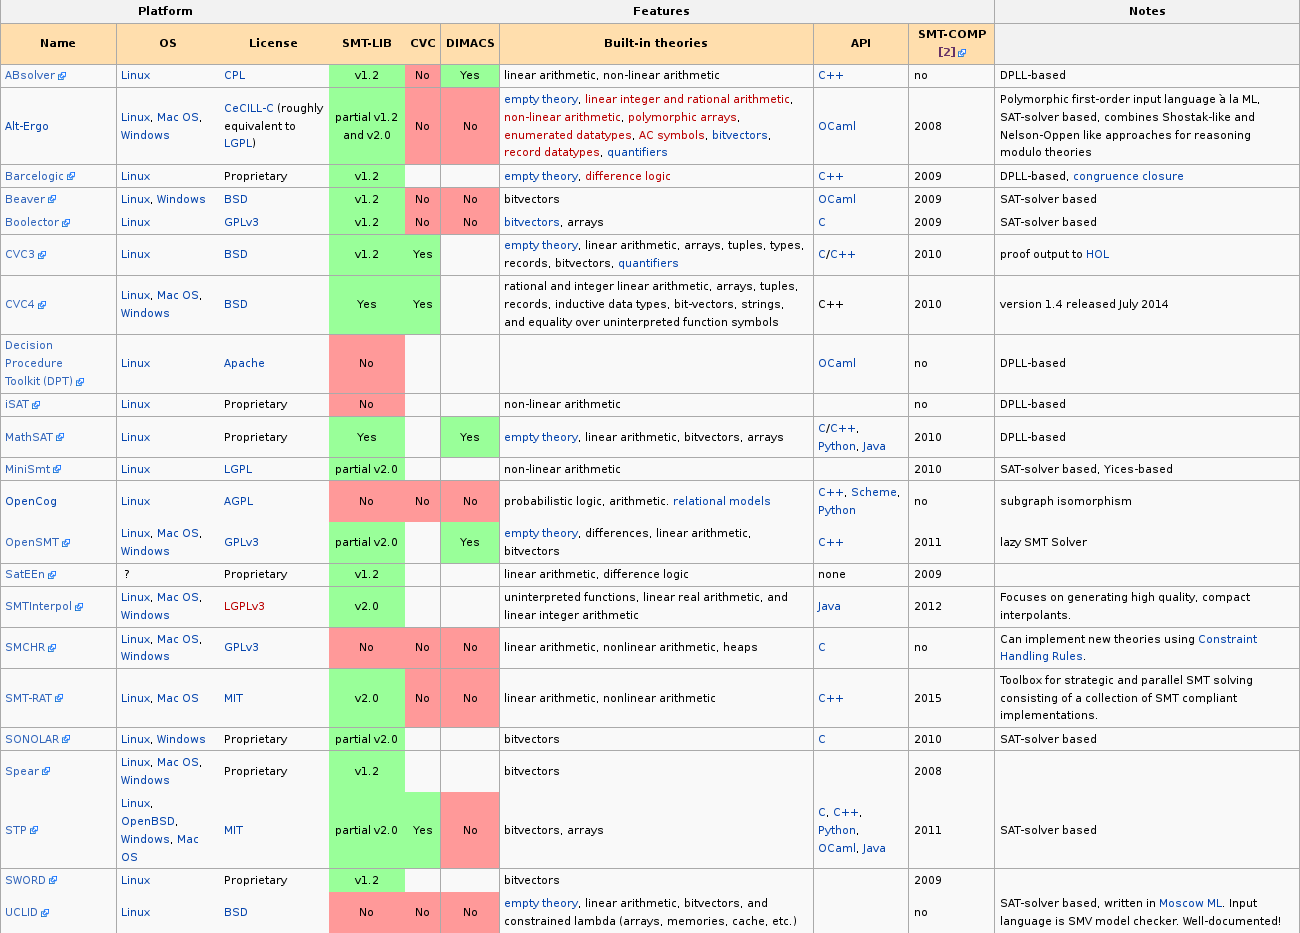
\includegraphics{solvers.png}}
  \end{center}
  ... different strengths and logic support.
\end{frame}

\subsection{VC generation}
\begin{frame}{Why3 and WP}
  \begin{itemize}
  \item So - \spark/WhyML and SMTLIB are quite different
  \item Last step is to go from the intermediate language to
    verification conditions expressed in SMTLIB
  \end{itemize}
\end{frame}

\begin{frame}{Why3 and WP}
  Why3 is a general purpose intermediate language:
  \begin{center}
    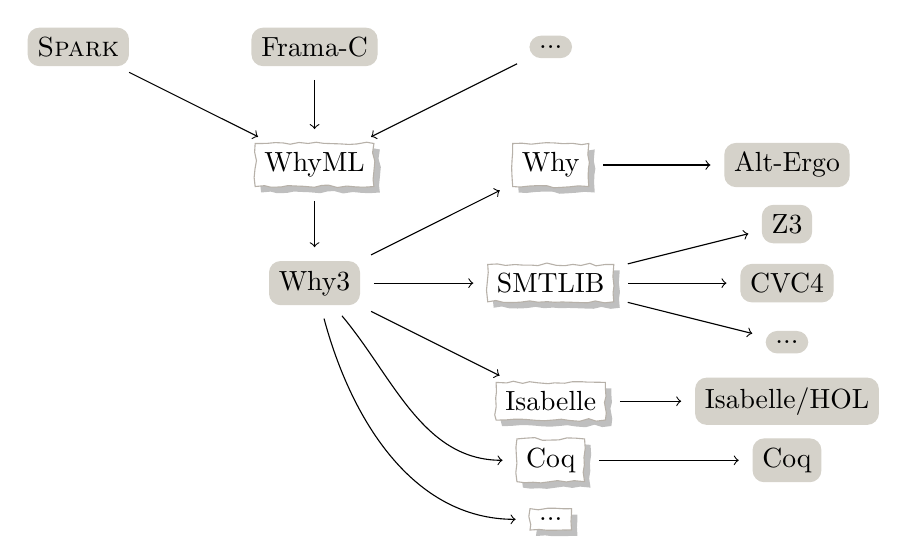
\begin{tikzpicture}[x=3cm,y=1.5cm,sa]
      \node[tool]  (spark)      at (-1, 2) {\spark};
      \node[tool]  (framac)     at (0, 2) {Frama-C};
      \node[tool]  (othertool)  at (1, 2) {...};

      \node[files] (whyml)    at (0,  1) {WhyML};

      \node[tool]  (gnatwhy3) at (0, 0) {Why3};

      \node[files] (smtlib)     at (1, 0) {SMTLIB};
      \node[files] (why)        at (1, 1) {Why};
      \node[files] (isabelle)   at (1, -1) {Isabelle};
      \node[files] (coqinput)   at (1, -1.5) {Coq};
      \node[files] (otherinput) at (1, -2) {...};

      \node[tool]  (cvc4) at (2, 0) {CVC4};
      \node[tool]  (z3) at (2, 0.5) {Z3};
      \node[tool]  (othersmt) at (2, -0.5) {...};
      \node[tool]  (altergo) at (2, 1) {Alt-Ergo};
      \node[tool]  (hol) at (2, -1) {Isabelle/HOL};
      \node[tool]  (coq) at (2, -1.5) {Coq};

      \draw[->] (spark) -- (whyml);
      \draw[->] (framac) -- (whyml);
      \draw[->] (othertool) -- (whyml);

      \draw[->] (whyml) -- (gnatwhy3);
      \draw[->] (gnatwhy3) -- (smtlib);
      \draw[->] (gnatwhy3) -- (why);
      \draw[->] (gnatwhy3) -- (isabelle);
      \draw[->] (gnatwhy3) to [out=-50, in=180] (coqinput);
      \draw[->] (gnatwhy3) to [out=-75, in=180] (otherinput);
      \draw[->] (smtlib) -- (cvc4);
      \draw[->] (smtlib) -- (z3);
      \draw[->] (smtlib) -- (othersmt);
      \draw[->] (why) -- (altergo);
      \draw[->] (isabelle) -- (hol);
      \draw[->] (coqinput) -- (coq);
    \end{tikzpicture}
  \end{center}
\end{frame}

\begin{frame}[fragile]{Why3 and WP}
  Consider Hoare triplets:
  \begin{itemize}
  \item<1-> $\{ precondition \}$ statement $\{ postcondition \}$
  \item<2-> $\{ \top \}$ \verb|x := 42| $\{ \top \}$
  \item<3-> $\{ \top \}$ \verb|x := 42| $\{ x > 0 \}$
  \item<4-> $\{ \top \}$ \verb|x := 42| $\{ x = 42 \}$
  \item<5-> $\{ \bot \}$ \verb|x := 42| $\{ x = 5 \}$
  \item<6-> $\{ x > 0 \}$ \verb|z := x + y| $\{ z > y \}$
  \end{itemize}
\end{frame}

\begin{frame}[fragile]{Why3 and WP}
  Consider this example:
  \begin{pxcode}[language=SPARK,gobble=4]
    -- precondition: $1 \leq a \leq 10$
    v1 := a + 5;
    v2 := v1 / 2;
    -- postcondition $1 \leq v2 \leq 10$
  \end{pxcode}

  \begin{block}{Weakest Precondition}
    $\{
    \only<3>{1 \leq a \leq 10 \implies -3 \leq a \leq 15}
    \only<5>{1 \leq a \leq 10 \implies 1 \leq (a + 5) / 2 \leq 10}
    \}$\\
    v1 := a + 5;\\
    $\{
    \only<2-3>{1 \leq a \leq 10 \implies 2 \leq v_1  \leq 20}
    \only<4->{1 \leq a \leq 10 \implies 1 \leq v_1 / 2 \leq 10}
    \}$\\
    v2 := v1 / 2;\\
    $\{
    1 \leq a \leq 10 \implies 1 \leq v_2 \leq 10
    \}$
  \end{block}
\end{frame}

\begin{frame}[fragile]{Why3 and WP}
  We've had this: $1 \leq a \leq 10 \implies 1 \leq (a + 5) / 2 \leq
  10$ \pause
  \begin{block}{example.smt2}
  \begin{pxcode}[language=SMTLIB,gobble=4]
    (set-logic QF_LIA)
    (declare-const a Int)
    (assert (<= 1 a 10))
    (assert (not (<= 1 (/ (+ a 5) 2) 10)))
    (check-sat)
  \end{pxcode}
  \end{block}
  \pause
  \begin{block}{Running CVC4...}
    \$ cvc4 example.smt2\\
    unsat
  \end{block}
  ... postcondition \structure{proven}!
\end{frame}

\begin{frame}{Why3 and WP}
  But programs are a bit more complicated...
  \begin{itemize}
  \item $\{ ? \}$ if a then x := y; $\{ x > 0 \}$
  \pause
  \item $\{ (\lnot a \implies x > 0) \land (a \implies y > 0) \}$\\
    if a then x := y;\\
    $\{ x > 0 \}$
  \pause
  \item ...or split in graph, producing 2 VCs
  \item (but this means exponential explosion)
  \end{itemize}
\end{frame}

\begin{frame}{Why3 and WP}
  Loops are the \structure{main issue}:
  \begin{itemize}
  \item $\{ P \}$ while c do s $\{ Q \}$
  \pause
  \item Requires a loop invariant $I$, which is \structure{difficult} to find
  \item Split into three VCs:
  \end{itemize}

  \begin{center}
    \begin{tikzpicture}[sa,y=1.5cm]
      \node (start) at (0, 2) {$P \implies I$};
      \node (loop)  at (0, 1) {while c do s};
      \node (end)   at (0, 0) {$I \land \lnot c \implies Q$};

      \draw[->] (start) -- (loop);
      \draw[->] (loop) -- (end);
      \draw[->] (loop.south east)
                to[out=-45,in=-90]
                (3, 1) node[auto,anchor=west] {$\{ I \land c \}$ s $\{ I \}$}
                to[out=90,in=45]
                (loop.north east);

    \end{tikzpicture}
  \end{center}
\end{frame}

\begin{frame}[fragile]{Why3 and WP}{Loop invariant example}
  \begin{pxcode}[language=SPARK,gobble=3]
   procedure Find_Element (A     : in     Int_Array;
                           Elem  : in     Integer;
                           Idx   :    out Natural;
                           Found :    out Boolean)
   with
      Global => null,
      Post   => (if Found
                 then A (Idx) = Elem
                 else (for all J in A'Range => A (J) /= Elem))
   is
   begin
      for I in A'Range loop
         Idx   := I;
         Found := A (I) = Elem;
         exit when Found;
         pragma Loop_Invariant
           ((for all J in A'First .. I => A (J) /= Elem)
            and not Found);
      end loop;
   end Find_Element;
  \end{pxcode}
\end{frame}


%%%%%%%%%%%%%%%%%%%%%%%%%%%%%%%%%%%%%%%%%%%%%%%%%%%%%%%%%%%%%%%%%%%%%%%%%%%%%%
\section{Conclusion}
\begin{frame}{Conclusion}
  Today we've seen:
  \begin{itemize}
  \item Architecture of modern static analysis systems:\\
    Source $\rightarrow$ Intermediate Language $\rightarrow$ SMTLIB
  \item Overview of \spark\ tool-set architecture
  \item Brief introduction to SMT
  \item Brief introduction to WP
  \item How this all comes together in \spark 2014
  \end{itemize}
  \pause
  \begin{center}
    Thank you for your time and attention.\\
    Also, we're hiring!\\
    Any questions?\\
  \end{center}
  \begin{center}
    \scriptsize Made using only Free Software.
  \end{center}
\end{frame}

\end{document}
